\documentclass[theoretical-framework.tex]{subfiles}
\usepackage[utf8]{inputenc}
\usepackage{graphicx}
\usepackage[
backend=biber,
style=alphabetic,
sorting=ynt
]{biblatex}


\addbibresource{references.bib} %Imports bibliography file


\title{Tecnologías Blockchain}
\author{Rocío Mena}
\date{\today}

\begin{document}

\section{Tecnología Blockchain}

La tecnología blockchain es una tecnología de base de datos distribuída. Esta estructura de datos distribuida mantiene un registro inmutable de transacciones o eventos validados mediante técnicas criptográficas que protegen los datos contra la manipulación. La información de esta base de datos se organiza en transacciones, que son validadas y agrupadas en bloques. Cada bloque, junto con un puntero al bloque anterior, forma una cadena de transacciones interconectadas criptográficamente. Una vez que una transacción se ha añadido a la cadena, generalmente no puede ser modificada ni eliminada porque requeriría cambiar todos los bloques posteriores en la cadena, lo cual es computacionalmente impracticable debido a la distribución y la seguridad criptográfica de la red blockchain. En la Figura \ref{fig:blockchain} se muestra un esquema de cómo se procesa una transacción en una blockchain.

\begin{figure}[h]
	\centering
	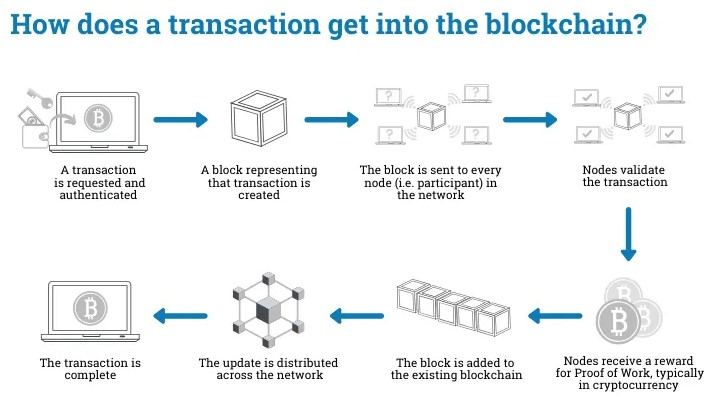
\includegraphics[width=0.8\textwidth]{./assets/blockchain.jpg}
	\caption{Funcionamiento de una transacción en una blockchain. Fuente: Ameen Alam, Medium.}
	\label{fig:blockchain}
\end{figure}

Esta arquitectura dota a la tecnología blockchain de características como inmutabilidad, transparencia y trazabilidad, que la convierten en una herramienta ideal para la gestión sostenible de la cadena de suministro. La tecnología blockchain ha sido ampliamente adoptada en diversos sectores y aplicaciones, incluyendo la trazabilidad de la cadena de suministro, la autenticación de productos, la gestión de identidad, la votación electrónica, la gestión de activos digitales y la creación de contratos inteligentes.

En este trabajo se analizan y comparan cinco tecnologías blockchain líderes en la industria: Hyperledger Fabric, Ethereum, Polkadot, VeChain y Cardano. Cada una de estas tecnologías tiene sus propias características, ventajas y desventajas, y es importante comprender sus diferencias para seleccionar la tecnología más adecuada para este caso de uso específico.

Cada tecnología se compara en distintos aspectos clave relevantes para este trabajo. Como el tipo de tecnología, el protocolo de consenso, el lenguaje de programación, la interoperabilidad, la adopción real y el tamaño de la comunidad. A continuación, se presenta una descripción detallada de cada tecnología y una comparación de sus características.

\subsection{Hyperledger Fabric}

Hyperledger Fabric es una plataforma de tecnología ledger distribuida (DLT) de código abierto y diseñada para uso en contextos empresariales \footnote{https://hyperledger-fabric.readthedocs.io/en/latest/index.html}. Hyperledger se estableció bajo la Fundación Linux y su sólida comunidad \cite{androulaki2018hyperledger}. 

Fabric tiene una arquitectura altamente modular y configurable, que permite la innovación, la versatilidad y la optimización para una amplia gama de casos de uso de la industria, incluida la cadena de suministro. Esta es la primera plataforma de ledger distribuida que admite contratos inteligentes creados en lenguajes de programación de uso general como Java, Go y Node.js, en lugar de lenguajes específicos de dominio restringidos (DSL). Esto significa que en la mayoría de los casos no requiere capacitación adicional para aprender un nuevo idioma para desarrollo de contratos inteligentes.

La plataforma Fabric también es permisionada, lo que significa que, a diferencia de una red pública sin permiso, los participantes se conocen entre sí, en lugar de ser anónimos y, por lo tanto, no se confía en absoluto. A su vez la plataforma tiene compatibilidad con protocolos de consenso conectables que permiten que la plataforma se personalice de manera más eficaz para adaptarse a casos de uso particulares y modelos de confianza. 

Fabric puede aprovechar los protocolos de consenso que no requieren una criptomoneda nativa para incentivar la minería costosa o impulsar la ejecución de contratos inteligentes. Evitar una criptomoneda reduce algunos vectores de riesgo / ataque significativos, y la ausencia de operaciones de minería criptográfica significa que la plataforma se puede implementar con aproximadamente el mismo costo operativo que cualquier otro sistema distribuido.

La combinación de estas características diferenciadoras de diseño convierte a Fabric en una de las plataformas de mejor rendimiento disponibles en la actualidad tanto en términos de procesamiento de transacciones como de latencia de confirmación de transacciones, y permite privacidad y confidencialidad de transacciones y los contratos inteligentes que los implementan.

\subsection{Ethereum}

Ethereum es una plataforma de código abierto basada en blockchain que permite a los desarrolladores crear y desplegar contratos inteligentes y aplicaciones descentralizadas (dApps) \footnote{https://ethereum.org/en/learn/}. Ethereum tiene como objetivo ser una computadora mundial descentralizada que ejecute cualquier tipo de aplicación. Esta plataforma es alimentada por su criptomoneda nativa, Ether, que se utiliza para pagar las transacciones y los servicios de la red \cite{buterin2013ethereum}.

Esta plataforma fue pionera en la creación de contratos inteligentes y ha sido un líder en la industria desde su lanzamiento en 2015. Ethereum es una plataforma de blockchain pública y sin permiso, lo que significa que cualquiera puede unirse a la red y participar en la validación de transacciones y la ejecución de contratos inteligentes. 

Los contratos inteligentes en Ethereum se escriben en Solidity \cite{dannen2017introducing}, un lenguaje de programación específico de dominio que se utiliza para definir las reglas y la lógica de una aplicación descentralizada. Los contratos inteligentes en Ethereum se ejecutan en la máquina virtual Ethereum (EVM), que es una máquina virtual Turing completa que puede ejecutar cualquier tipo de código. El lenguaje Solidity está inspirado en JavaScript y C++, lo que facilita su aprendizaje para los desarrolladores que ya están familiarizados con estos lenguajes.

Ethereum utiliza un protocolo de consenso de prueba de trabajo (PoW, Proof of Work) para validar las transacciones y agregar nuevos bloques a la cadena de bloques. Sin embargo, Ethereum está en proceso de migrar a un protocolo de consenso de prueba de participación (PoS, Proof of Stake). 

\subsection{Polkadot}

Polkadot es una plataforma de blockchain de código abierto que permite la interoperabilidad entre diferentes blockchains \footnote{https://polkadot.network/}. Polkadot tiene como objetivo crear una red de blockchain escalable, segura e interoperable que pueda soportar una amplia gama de aplicaciones descentralizadas y contratos inteligentes. Esta plataforma es desarrollada por la Web3 Foundation y posee una sólida comunidad de desarrolladores activos \cite{wood2016polkadot}.

La arquitectura de esta plataforma consta de una cadena principal ("Relay Chain") y múltiples cadenas que se conectan a ella ("parachains"). Cada parachain es una blockchain independiente, pero puede comunicarse con las demás blockchains a través de la cadena principal. Esto permite que las aplicaciones descentralizadas y los contratos inteligentes se ejecuten en diferentes blockchains y se comuniquen entre sí de manera eficiente. 

Esta plataforma utiliza un protocolo de consenso de PoS llamado "Nominated Proof of Stake" (NPoS) para validar las transacciones y agregar nuevos bloques a la cadena de bloques. La red posee una criptomoneda nativa llamada DOT, que se utiliza para pagar las transacciones y los servicios de la red. Cada blockchain en Polkadot puede tener su propia criptomoneda nativa y su propio conjunto de reglas y lógica.

Las aplicaciones para Polkadot son desarrolladas utilizando Substrate \footnote{https://docs.substrate.io/}, un framework modular escrito en Rust que facilita la creación de blockchains personalizadas y parachains. Substrate también posee un módulo de compatibilidad con contratos inteligentes escritos en Solidity, el lenguaje de programación utilizado en Ethereum.

\subsection{VeChain}

VeChain es una plataforma de blockchain de código abierto dedicada a la trazabilidad y que busca asegurar la autenticidad de los productos en la cadena de suministro \footnote{https://docs.vechain.org/introduction-to-vechain/about-the-vechain-blockchain}. VeChain utiliza una combinación de tecnología blockchain, RFID e Internet de las cosas (IoT) para rastrear el movimiento de productos a lo largo de toda la cadena de suministro, desde la producción hasta el consumidor final. Esta plataforma es desarrollada por la Fundación VeChain y tiene como objetivo mejorar la transparencia y la confianza en la cadena de suministro \cite{she2022vechain}.

VeChain es una plataforma permisionada, lo que significa que los participantes de la red se conocen entre sí y se confían mutuamente. Esto permite una mayor privacidad y confidencialidad de las transacciones y los contratos inteligentes que se ejecutan en la red. VeChain también utiliza una tecnología de identificación por radiofrecuencia (RFID) para rastrear los productos a lo largo de la cadena de suministro y garantizar su autenticidad.

Esta plataforma utiliza una arquitectura de dos tokens, donde VET es la criptomoneda nativa utilizada para pagar las transacciones y los servicios de la red, y VTHO es un token secundario utilizado para pagar el costo de la ejecución de contratos inteligentes y las transacciones en la red. Esta plataforma utiliza un protocolo de consenso de PoS llamado prueba de autoridad (PoA, Proof of Authority) para validar las transacciones y agregar nuevos bloques a la cadena.

Las aplicaciones para VeChain pueden desarrollarse utilizando el lenguaje de programación Solidity, el mismo utilizado en Ethereum, lo que facilita la migración de aplicaciones existentes de Ethereum a VeChain. A su vez, también se pueden desarrollar aplicaciones personalizadas utilizando el framework de desarrollo de Smart Contracts de VeChain, que proporciona una serie de herramientas y bibliotecas para facilitar el desarrollo de aplicaciones descentralizadas y contratos inteligentes.

\subsection{Cardano}

Cardano es una plataforma de blockchain de código abierto que busca crear una red de blockchain escalable, segura y sostenible \footnote{https://docs.cardano.org/about-cardano/introduction/\#cardano-explained}. Cardano tiene como objetivo ser una plataforma de contratos inteligentes de tercera generación que pueda soportar una amplia gama de aplicaciones descentralizadas y contratos inteligentes. Cardano se caracteriza por su enfoque científico y riguroso en su desarrollo, utilizando evidencia formal y revisión por pares para garantizar la seguridad y confiabilidad de la plataforma \cite{hoskinson2017we}.

Una de las características distintivas de Cardano es su enfoque en la seguridad y la provisión de garantías formales. Para programar aplicaciones en esta plataforma se utiliza el lenguaje de programación funcional Haskell, que permite la verificación formal de contratos inteligentes y protocolos. También se pueden desarrollar contratos inteligentes utilizando Plutus \cite{chakravarty2019functional}\footnote{https://developers.cardano.org/docs/smart-contracts/plutus/}, un lenguaje de programación específico de dominio basado en Haskell que facilita la creación de contratos inteligentes seguros y confiables en Cardano.

Esta plataforma utiliza un protocolo de consenso de PoS, que es más eficiente energéticamente que los protocolos de PoW. La red posee una criptomoneda nativa llamada ADA, que se utiliza para pagar las transacciones y los servicios de la red.

\subsection{Comparación de tecnologías}

A continuación se realiza una comparación de las tecnologías blockchain mencionadas anteriormente en términos de tipo de tecnología, protocolo de consenso, lenguaje de programación, interoperabilidad, adopción real y tamaño de la comunidad.

\begin{table}[h!]
	\centering
	\begin{tabular}{|c|c|c|c|c|c|}
	\hline
	\textbf{Tecnología} \textbf{Hyperledger} & \textbf{Ethereum} & \textbf{Polkadot} & \textbf{VeChain} & \textbf{Cardano} \\ \hline
	\\ \hline
	Tipo & Pública & Pública & Pública & Permisionada & Pública \\ \hline
	Consenso & Pluggable & PoW - PoS & PoS & PoA & PoS \\ \hline
	Lenguaje & Java, Go, Node.js & Solidity & Rust, Solidity & Solidity & Haskell \\ \hline
	Interoperabilidad & Limitada & Limitada & Alta & Limitada & Limitada \\ \hline
	Adopción & Alta & Muy alta & Media & Media & Media \\ \hline
	Comunidad & Grande & Grande & Grande & Mediana & Grande \\ \hline
\end{tabular}
\caption{Comparación de plataformas blockchain}
\end{table}

\subsection{Conclusión}


En base al análisis realizado es los distintos aspectos clave de cada plataforma, se elige a Ethereum como la tecnología blockchain más adecuada para el desarrollo de este trabajo por los siguientes motivos:

\begin{itemize}
	\item Pública: Ethereum es una plataforma de blockchain pública y sin permiso, lo que permite a cualquier persona unirse a la red, leer el estado de la cadena de bloques y participar en la validación de transacciones.
	\item PoS: en su última actualización, Ethereum está migrando a un protocolo de consenso de prueba de participación, que es más eficiente energéticamente que el protocolo de PoW, por lo que es más sostenible a largo plazo y reduce el impacto ambiental del uso de la aplicación.
	\item Comunidad: entre las opciones revisadas, Ethereum posee la mayor comunidad de desarrolladores activos y adopción en la industria, lo que garantiza un soporte continuo y una amplia gama de recursos disponibles durante el desarrollo y mantenimiento de la aplicación. 
	\item Lenguaje de programación: Ethereum utiliza el lenguaje de programación Solidity para desarrollar contratos inteligentes y aplicaciones descentralizadas. Este lenguaje de alto nivel es fácil de aprender y permite a los desarrolladores crear aplicaciones complejas de manera eficiente.
	\item Interoperabilidad: Ethereum es compatible con una amplia gama de aplicaciones y protocolos, lo que facilita la interoperabilidad con otras plataformas de blockchain y aplicaciones descentralizadas. De entre las opciones revisadas, Ethereum es la plataforma más compatible y versátil para integrar con otras tecnologías y sistemas y posee una amplia gama de herramientas y bibliotecas disponibles para facilitar la integración.
\end{itemize}

\end{document}
